\chapter{Energy and the Hamiltonian}

\lectureoverview{We first sharpen the meaning of an active symmetry and
review how translations and rotations generate momentum and angular momentum.
The missing conservation law is energy.  Its symmetry is translation in time,
and its conserved quantity is the Hamiltonian
\(H=\sum_i p_i\dot q_i-L\).  The derivation also shows exactly how explicit
time dependence transfers energy between a chosen subsystem and its
environment.}

\section{Questions Before the Formal Argument}

We are approaching the absolute minimum of classical mechanics needed for the
subjects that follow, though there is still much more mechanics worth
learning.  Two questions arose before the main argument began.

\begin{classroomqa}
  \audiencequestion{Which books are useful after this introductory course?
  \lecturetimestamp{00:00:36--00:02:13}}
  \lecturerresponse{The established advanced reference is Herbert
  Goldstein's \emph{Classical Mechanics}.  Cornelius Lanczos's book on the
  variational principles of mechanics is another relevant source.  A class
  reading list is more useful than pretending that one lecturer can survey
  every available text.}
\end{classroomqa}

The second question records a moment in the history of an unresolved
measurement.  In 2011 the OPERA experiment had reported an apparent early
arrival of neutrinos sent from CERN to Gran Sasso.  The reported discrepancy
was shorter than the proton pulse used to create the neutrinos, so the timing
analysis depended on comparing pulse profiles rather than tagging one
neutrino at emission and recognizing the same particle at detection.

\begin{classroomqa}
  \audiencequestion{Had the apparent faster-than-light neutrino result been
  resolved?
  \lecturetimestamp{00:02:30--00:09:03}}
  \lecturerresponse{No conclusion was then justified.  Beam-pulse shape,
  target heating, and synchronization all demanded technical scrutiny.  One
  speculative proposal considered the motion of a GPS satellite: in the
  satellite frame the source and detector move while timing signals travel,
  producing corrections of order tens of nanoseconds.  The estimate was
  interesting as an order-of-magnitude exercise, but it was not presented as
  a believable diagnosis of the experiment.  Ordinary Lorentz contraction at
  the relevant speed was too small to supply the reported effect.  The proper
  response was to wait for the experimental analysis.}
\end{classroomqa}

\begin{figure}[htbp]
  \centering
  
\includegraphics[width=0.78\textwidth]{lecture_05_figure_07.png}
  \caption{The satellite-frame timing sketch discussed during the historical
  neutrino-measurement question.}
  \lectureframe{00:06:30}
\end{figure}

The timing discussion is not needed for the mechanics below.  It is useful
nevertheless as a reminder that a plausible scale estimate is not the same as
an established experimental explanation.

\section{Active Symmetry and the Choice of System}

Let us return to the point that was left too blurred in the preceding
discussion: what precisely is a symmetry?  Consider a particle on a line and
the instruction
\begin{equation}
  x\longrightarrow x+1.
  \label{eq:l5-shift-one}
\end{equation}
There are two ways to understand it.  A \emph{passive} transformation relabels
the points of the line.  A point once called \(x=0\) may now be called
\(x'=1\), but the particle has not moved.  An \emph{active} transformation
keeps the labels fixed and moves the particle itself from \(x\) to \(x+1\).
Only the second operation changes its position relative to an external
potential.

\begin{figure}[htbp]
  \centering
  
\includegraphics[width=0.82\textwidth]{lecture_05_figure_08.png}
  \caption{The rule \(x\mapsto x+1\), the fixed coordinate line, and an
  external potential distinguish active motion from passive relabeling.}
  \lectureframe{00:11:20}
\end{figure}

\begin{classroomqa}
  \audiencequestion{If moving the particle changes its potential energy, is
  the source of that potential being excluded from the system?
  \lecturetimestamp{00:12:19--00:14:18}}
  \lecturerresponse{Exactly.  Calling the system ``a particle in a
  potential'' divides the world into the particle and a heavy environment,
  such as the Earth, that produces \(V(x)\).  The Earth does recoil, but its
  enormous mass makes that recoil negligible in this approximation.  Moving
  the particle relative to the fixed Earth can change \(V\); translating the
  particle and Earth together would not.}
\end{classroomqa}

\begin{classroomqa}
  \audiencequestion{In the earlier rotation example, were the velocities
  changed as well as the positions?
  \lecturetimestamp{00:14:26--00:15:29}}
  \lecturerresponse{Yes.  A rigid active rotation acts on the entire history,
  not on one instantaneous position alone.  Positions and velocity vectors
  are both rotated.  By contrast, a constant translation applied at every
  time changes \(x\) but leaves \(\dot x\) unchanged.}
\end{classroomqa}

The distinction between system and environment will return twice: when a
time-dependent apparatus exchanges energy with a subsystem, and when
macroscopic friction hides energy in unobserved microscopic motion.

\section{Infinitesimal Motions in Configuration Space}

A configuration of a general mechanical system is a point in the space of
generalized coordinates \(q_i\).  An active infinitesimal transformation moves
every possible configuration to a nearby one.  We write
\begin{equation}
  \delta q_i=\epsilon f_i(q),
  \label{eq:l5-general-transformation}
\end{equation}
where the functions \(f_i\) specify one fixed displacement field on
configuration space.  They may depend on all the coordinates and some may
vanish.  The common factor \(\epsilon\) is small; it separates the size of the
step from the shape of the transformation.

\begin{figure}[htbp]
  \centering
  
\includegraphics[width=0.75\textwidth]{lecture_05_figure_09.png}
  \caption{A displacement vector attached to each point of configuration
  space.}
  \lectureframe{00:16:50}
\end{figure}

\begin{figure}[htbp]
  \centering
  
\includegraphics[width=0.80\textwidth]{lecture_05_figure_10.png}
  \caption{The coordinate-dependent infinitesimal transformation
  \(\delta q_i=\epsilon f_i(q)\).}
  \lectureframe{00:18:00}
\end{figure}

The rule itself has no explicit time dependence.  Its action on velocities is
therefore
\begin{equation}
  \delta\dot q_i=\frac{d}{dt}(\delta q_i)
  =\epsilon\sum_j\frac{\partial f_i}{\partial q_j}\dot q_j.
  \label{eq:l5-velocity-variation}
\end{equation}
For a translation, \(f_x=1\), so \(\delta\dot x=0\).  For a rotation,
\(f_i\) depends on position, and the velocity changes.

\begin{classroomqa}
  \audiencequestion{Is the final small factor in
  \(\delta q_i=\epsilon f_i(q)\) the same constant at every point?
  \lecturetimestamp{00:19:58--00:20:51}}
  \lecturerresponse{Yes.  The single constant \(\epsilon\) is a bookkeeping
  device that makes all coordinate changes first order in the same small
  quantity.  The functions \(f_i(q)\), not \(\epsilon\), contain the spatial
  dependence and need not themselves be small.}
\end{classroomqa}

\section{What Makes the Transformation a Symmetry?}

An active transformation generally changes the potential energy.  It can also
change the kinetic energy.  In curvilinear coordinates the kinetic term has
the form
\begin{equation}
  T=\frac12\sum_{i,j}g_{ij}(q)\dot q_i\dot q_j,
  \label{eq:l5-kinetic-metric}
\end{equation}
so moving in configuration space can change its coefficients.  The familiar
\(r^2\dot\theta^2\) term in polar coordinates is the simplest example.

A transformation is a symmetry here when the \emph{whole} Lagrangian has no
first-order change,
\begin{equation}
  \delta L=O(\epsilon^2),
  \label{eq:l5-symmetry-condition}
\end{equation}
and this must hold at every point of configuration space, not only at the
configuration occupied by one particular solution.

For example, under \(x\mapsto x+\epsilon\),
\begin{equation}
  \delta V=\frac{\partial V}{\partial x}\epsilon.
  \label{eq:l5-potential-variation}
\end{equation}
If this vanishes for every possible \(x\), then
\(\partial V/\partial x=0\): the potential is independent of \(x\).  If it is
unchanged under translations in every spatial direction, it is constant.

\begin{figure}[htbp]
  \centering
  
\includegraphics[width=0.80\textwidth]{lecture_05_figure_11.png}
  \caption{An \(x\)-translation tested against a potential \(V(y)\) that is
  independent of \(x\).}
  \lectureframe{00:23:40}
\end{figure}

For a smooth one-parameter family, the vanishing first-order change at every
point lets us compose infinitesimal steps into a finite symmetry.

\begin{classroomqa}
  \audiencequestion{Must kinetic and potential energy remain invariant
  separately?
  \lecturetimestamp{00:24:44--00:25:33}}
  \lecturerresponse{No.  Only the total Lagrangian must be invariant.  Some
  Lagrangians contain mixed coordinate--velocity terms and do not admit a
  useful separation into \(T\) and \(V\), so separate invariance may not even
  be a meaningful question.}
\end{classroomqa}

\begin{classroomqa}
  \audiencequestion{Does ``no change'' mean exactly no change, or merely a
  change small enough to neglect?
  \lecturetimestamp{00:25:34--00:28:59}}
  \lecturerresponse{For an infinitesimal transformation it means no term
  proportional to \(\epsilon\).  Terms of order \(\epsilon^2\) are discarded in
  the local calculation.  Because the first-order condition holds everywhere
  along the one-parameter orbit, repeating the local step yields the finite
  invariance.}
\end{classroomqa}

\section{Momentum and Angular Momentum Recovered}

For the exact, time-independent point symmetries considered here, the result
proved previously is
\begin{equation}
  Q=\sum_i p_i f_i(q),
  \qquad
  p_i=\frac{\partial L}{\partial\dot q_i},
  \qquad
  \dot Q=0.
  \label{eq:l5-noether-charge}
\end{equation}
The factor \(\epsilon\) does not belong in \(Q\); it measures only how far we
move along the symmetry orbit.

\begin{figure}[htbp]
  \centering
  
\includegraphics[width=0.82\textwidth]{lecture_05_figure_12.png}
  \caption{The general infinitesimal displacement and its conserved Noether
  charge.}
  \lectureframe{00:30:00}
\end{figure}

For a translation in \(x\), \(f_x=1\), and \(Q=p_x\).  Full translation
invariance gives conservation of all three components of momentum.  For many
interacting particles, the symmetry translates every particle together, so
\begin{equation}
  \mathbf P=\sum_a\mathbf p_a
  \label{eq:l5-total-momentum}
\end{equation}
is conserved when the interactions depend only on relative positions.  Moving
one particle relative to the rest is not the symmetry.

\begin{figure}[htbp]
  \centering
  
\includegraphics[width=0.80\textwidth]{lecture_05_figure_13.png}
  \caption{A common translation produces conservation of total momentum,
  component by component.}
  \lectureframe{00:32:50}
\end{figure}

For an infinitesimal rotation in the \(x\)-\(y\) plane, choose the orientation
\begin{equation}
  \delta x=-y\epsilon,
  \qquad
  \delta y=x\epsilon.
  \label{eq:l5-planar-rotation}
\end{equation}
It preserves the radius because
\begin{equation}
  \delta(x^2+y^2)
  =2x\delta x+2y\delta y=0.
  \label{eq:l5-radius-invariance}
\end{equation}

\begin{figure}[htbp]
  \centering
  
\includegraphics[width=0.76\textwidth]{lecture_05_figure_14.png}
  \caption{The geometry and coordinate formula for an infinitesimal planar
  rotation.}
  \lectureframe{00:35:05}
\end{figure}

Differentiating Eq.~\eqref{eq:l5-planar-rotation} rotates the velocities as
well.  Thus \(\dot x^2+\dot y^2\) is invariant, and a central potential
\(V(\sqrt{x^2+y^2})\) leaves the complete Lagrangian unchanged.  The charge is
\begin{equation}
  Q=-yp_x+xp_y=(\mathbf r\times\mathbf p)_z.
  \label{eq:l5-angular-charge}
\end{equation}

\begin{figure}[htbp]
  \centering
  
\includegraphics[width=0.76\textwidth]{lecture_05_figure_15.png}
  \caption{The rotational Noether charge, the \(z\)-component of angular
  momentum.}
  \lectureframe{00:38:50}
\end{figure}

Rotations in the other coordinate planes give the remaining components.  For
many particles the conserved vector is
\begin{equation}
  \mathbf J=\sum_a\mathbf r_a\times\mathbf p_a.
  \label{eq:l5-total-angular-momentum}
\end{equation}
A planet in a central stellar potential is the basic example: invariance under
all rotations implies conservation of all components of angular momentum.

\begin{classroomqa}
  \audiencequestion{What happens at a sharp cusp, where the derivative from
  one side differs from the derivative from the other?
  \lecturetimestamp{00:42:25--00:44:21}}
  \lecturerresponse{That is a legitimate qualification.  The present
  argument assumes differentiable functions with unique derivatives.  An
  unstable equilibrium, such as an object balanced at a smooth maximum, is
  not itself a problem: the derivative there exists and vanishes.  A literal
  cusp requires a modified treatment.}
\end{classroomqa}

\begin{classroomqa}
  \audiencequestion{If the transformation parameter is time independent,
  why does a rotation change the velocities?
  \lecturetimestamp{00:44:23--00:45:23}}
  \lecturerresponse{The parameter is constant, but the displacement field is
  coordinate dependent.  The universal rule is
  \(\delta\dot q_i=d(\delta q_i)/dt\).  A translation has constant
  \(\delta x\), whereas a rotation has \(\delta x=-y\epsilon\) and therefore
  \(\delta\dot x=-\dot y\epsilon\).}
\end{classroomqa}

\section{Beyond the Elementary Kinetic-minus-Potential Form}

In Cartesian coordinates for ordinary nonrelativistic particles without
magnetic fields, \(L=T-V\).  More general coordinates produce the quadratic
form of Eq.~\eqref{eq:l5-kinetic-metric}.  A magnetic field introduces a term
linear in velocity, schematically \(\mathbf A(q)\cdot\dot{\mathbf q}\), which
mixes coordinates and velocities.  In such a case it is better to treat
\(L(q,\dot q,t)\) as one function than to force every term into conventional
kinetic and potential boxes.

\begin{figure}[htbp]
  \centering
  
\includegraphics[width=0.80\textwidth]{lecture_05_figure_16.png}
  \caption{A general coordinate-dependent quadratic kinetic term beside a
  coordinate-only potential.}
  \lectureframe{00:47:20}
\end{figure}

\begin{classroomqa}
  \audiencequestion{Why might a Lagrangian fail to separate neatly into
  kinetic and potential energy, and is it still defined as \(T-V\)?
  \lecturetimestamp{00:45:26--00:48:13}}
  \lecturerresponse{The obstruction may come from curvilinear coordinates or
  from genuine velocity-dependent interactions such as magnetism.  Only when
  the Lagrangian consists of a quadratic velocity form minus a coordinate-only
  function do we name those pieces \(T\) and \(V\).  Otherwise the Lagrangian
  remains a perfectly good function of \(q\) and \(\dot q\), but the split is
  not profitable.  The correct general definition of energy will come from
  the Hamiltonian.}
\end{classroomqa}

\begin{classroomqa}
  \audiencequestion{Was the hanging-chain example from the first meeting an
  application of least action?
  \lecturetimestamp{00:48:15--00:49:45}}
  \lecturerresponse{It was an equilibrium problem governed by least energy,
  not a history selected by stationary action.  For a static solution of an
  ordinary \(T-V\) system, \(\dot p_i=0\) and the Euler--Lagrange equation
  reduces to \(\partial V/\partial q_i=0\), the condition for a stationary
  point of the potential.}
\end{classroomqa}

Momentum and angular momentum have now been tied to spatial symmetries.  The
conspicuous missing quantity is energy.

\section{Time Translation Invariance}

Imagine an experiment that starts at \(t_0\), ends at \(t_1\), and produces an
outcome.  Repeat the same preparation later, starting at
\(t_0+\Delta t\) and ending at \(t_1+\Delta t\).  If the outcome is unchanged,
the system is invariant under an active translation in time.

\begin{figure}[htbp]
  \centering
  
\includegraphics[width=0.82\textwidth]{lecture_05_figure_17.png}
  \caption{An experiment and its time-translated copy in configuration-space
  history.}
  \lectureframe{00:52:45}
\end{figure}

A charged particle between capacitor plates illustrates failure of this
symmetry.  With fixed plate charge, the same experiment can be performed at
any time.  If an external generator is steadily charging the plates, the
particle sees a different electric field depending on when it is released.
The particle is then an explicitly driven subsystem.

\begin{figure}[htbp]
  \centering
  
\includegraphics[width=0.82\textwidth]{lecture_05_figure_18.png}
  \caption{Fixed and externally changing capacitor plates contrasted beside
  the time-translation diagram.}
  \lectureframe{00:54:45}
\end{figure}

The same point appears in an oscillator,
\begin{equation}
  L=\frac12m\dot x^2-\frac12k(t)x^2.
  \label{eq:l5-driven-oscillator}
\end{equation}
An external electric or magnetic field might slowly alter the material and
hence its effective spring constant.  If \(k\) varies, shifting the oscillator
experiment in time changes the result.

\begin{figure}[htbp]
  \centering
  
\includegraphics[width=0.78\textwidth]{lecture_05_figure_19.png}
  \caption{The oscillator's kinetic and potential terms during the discussion
  of a time-dependent spring constant.}
  \lectureframe{00:56:45}
\end{figure}

If the apparatus that changes \(k\) is included in the system, the full closed
experiment can again be time translated and its full energy is conserved.
The apparent nonconservation is energy exchange across a boundary we chose.

During the break the small transformation parameter was renamed
\(\epsilon\), avoiding the visually confusing expression
\(\delta x=\delta\).  A class recommendation for a book about Emmy Noether was
also noted for the shared reading list.

\begin{classroomqa}
  \audiencequestion{If the Lagrangian is not given as \(T-V\), where does it
  come from?
  \lecturetimestamp{01:00:17--01:02:24}}
  \lecturerresponse{It may be inferred from experiment, reconstructed from
  known equations of motion, guessed from symmetry and other theoretical
  principles, or found by trial and error.  Once \(L(q,\dot q,t)\) is given,
  the Euler--Lagrange calculus turns it into equations of motion.  The formal
  argument does not require us to settle its origin first.}
\end{classroomqa}

The operational test for time-translation invariance is now immediate.  If
knowledge of \(q\) and \(\dot q\) suffices to determine \(L\), without also
knowing the clock time, then
\begin{equation}
  \frac{\partial L}{\partial t}=0.
  \label{eq:l5-no-explicit-time}
\end{equation}
This does not say that \(L(q(t),\dot q(t))\) is constant along a motion.  It
says only that there is no time dependence beyond that carried by the evolving
coordinates and velocities.

A rotating heavy dumbbell provides another driven example.  If its prescribed
motion creates a time-varying gravitational potential for a light test
particle, the test-particle Lagrangian depends explicitly on time.  Treating
the dumbbell dynamically instead would enlarge the system and remove that
external time dependence.

\begin{figure}[htbp]
  \centering
  
\includegraphics[width=0.80\textwidth]{lecture_05_figure_20.png}
  \caption{A prescribed rotating dumbbell acts as a time-dependent external
  source for a lighter particle.}
  \lectureframe{01:06:25}
\end{figure}

\section{Deriving the Hamiltonian}

Suppose we did not know the formula for energy and guessed that perhaps the
Lagrangian itself were conserved.  The direct test is to differentiate it
along an actual trajectory.  Begin, for simplicity, with no explicit time
dependence:
\begin{equation}
  \frac{dL}{dt}
  =\sum_i\left(
    \frac{\partial L}{\partial q_i}\dot q_i
    +\frac{\partial L}{\partial\dot q_i}\ddot q_i
  \right).
  \label{eq:l5-chain-rule-no-time}
\end{equation}

\begin{figure}[htbp]
  \centering
  
\includegraphics[width=0.72\textwidth]{lecture_05_figure_02.png}
  \caption{Beginning the derivative of \(L(q_i,\dot q_i)\) along the
  trajectory.}
  \lectureframe{01:08:51}
\end{figure}

\begin{classroomqa}
  \audiencequestion{Is a summation missing from the chain-rule expression?
  \lecturetimestamp{01:10:39--01:11:05}}
  \lecturerresponse{Yes.  Every coordinate and every velocity can change the
  Lagrangian, so both terms are summed over \(i\).}
\end{classroomqa}

Use the canonical momentum and the Euler--Lagrange equation,
\begin{equation}
  p_i=\frac{\partial L}{\partial\dot q_i},
  \qquad
  \dot p_i=\frac{\partial L}{\partial q_i}.
  \label{eq:l5-p-and-pdot}
\end{equation}
Then Eq.~\eqref{eq:l5-chain-rule-no-time} becomes
\begin{align}
  \frac{dL}{dt}
  &=\sum_i(\dot p_i\dot q_i+p_i\ddot q_i)
  \notag\\
  &=\frac{d}{dt}\sum_i p_i\dot q_i.
  \label{eq:l5-product-rule}
\end{align}
The ``magic'' is only the product rule.

\begin{figure}[htbp]
  \centering
  
\includegraphics[width=0.84\textwidth]{lecture_05_figure_21.png}
  \caption{The chain rule converted, using the equations of motion, into the
  derivative of \(\sum_i p_i\dot q_i\).}
  \lectureframe{01:13:45}
\end{figure}

\begin{classroomqa}
  \audiencequestion{Should the final \(q_i\) in the product carry one dot or
  two?
  \lecturetimestamp{01:14:31--01:15:32}}
  \lecturerresponse{Inside the product it is \(p_i\dot q_i\), with one dot.
  Differentiating the product gives
  \(\dot p_i\dot q_i+p_i\ddot q_i\), which explains the two dots in the
  expanded second term.}
\end{classroomqa}

Subtracting the two derivatives gives a conserved combination.  Historical
convention chooses its negative and calls it the Hamiltonian:
\begin{equation}
  H=\sum_i p_i\dot q_i-L.
  \label{eq:l5-hamiltonian-definition}
\end{equation}

\begin{figure}[htbp]
  \centering
  
\includegraphics[width=0.80\textwidth]{lecture_05_figure_22.png}
  \caption{The conserved combination \(L-\sum_i p_i\dot q_i=-H\) and the
  Hamiltonian definition.}
  \lectureframe{01:18:05}
\end{figure}

For one particle in a potential,
\begin{equation}
  L=\frac12m\dot x^2-V(x),
  \qquad p=m\dot x.
  \label{eq:l5-particle-lagrangian}
\end{equation}
Therefore
\begin{align}
  H&=p\dot x-L
  \notag\\
   &=m\dot x^2-\left(\frac12m\dot x^2-V(x)\right)
  \notag\\
   &=\frac12m\dot x^2+V(x)=T+V.
  \label{eq:l5-particle-energy}
\end{align}

\begin{figure}[htbp]
  \centering
  
\includegraphics[width=0.86\textwidth]{lecture_05_figure_23.png}
  \caption{The Hamiltonian of a particle in a potential reduces to the
  familiar kinetic plus potential energy.}
  \lectureframe{01:20:50}
\end{figure}

The derivation did not assume a particular form of \(L\).  Thus
Eq.~\eqref{eq:l5-hamiltonian-definition}, rather than \(T+V\), is the general
definition of energy in this formalism.

\section{Explicit Time Dependence and Energy Exchange}

Restore explicit time dependence in the chain rule:
\begin{equation}
  \frac{dL}{dt}
  =\sum_i\left(
    \frac{\partial L}{\partial q_i}\dot q_i
    +\frac{\partial L}{\partial\dot q_i}\ddot q_i
  \right)
  +\frac{\partial L}{\partial t}.
  \label{eq:l5-full-chain-rule}
\end{equation}
The left side is the total derivative along the motion.  The final partial
derivative holds \(q\) and \(\dot q\) fixed and differentiates only externally
changing parameters.  Repeating the same product-rule step yields
\begin{equation}
  \boxed{\frac{dH}{dt}=-\frac{\partial L}{\partial t}}.
  \label{eq:l5-hamiltonian-time}
\end{equation}

\begin{figure}[htbp]
  \centering
  
\includegraphics[width=0.70\textwidth]{lecture_05_figure_04.png}
  \caption{The Hamiltonian changes only through explicit time dependence of
  the Lagrangian.}
  \lectureframe{01:37:22}
\end{figure}

For the driven oscillator of Eq.~\eqref{eq:l5-driven-oscillator},
\begin{equation}
  \frac{\partial L}{\partial t}
  =-\frac12\dot k(t)x^2,
  \qquad
  \dot H=\frac12\dot k(t)x^2.
  \label{eq:l5-driven-energy-rate}
\end{equation}
At \(x=0\) the instantaneous rate vanishes; away from the origin, changing the
spring constant does work at a rate proportional to \(x^2\dot k\).

\begin{classroomqa}
  \audiencequestion{If energy is not conserved, is its definition the time
  derivative of the Hamiltonian?
  \lecturetimestamp{01:27:11--01:28:04}}
  \lecturerresponse{No.  The energy is \(H\).  Its derivative tells us how
  that energy changes.  When the Lagrangian has the familiar form, \(H=T+V\);
  when it does not, Eq.~\eqref{eq:l5-hamiltonian-definition} supplies the
  definition.  Enlarging the system to include the external driver restores
  conservation of the total Hamiltonian.}
\end{classroomqa}

\begin{classroomqa}
  \audiencequestion{How does this apply to the earlier observer on a rotating
  merry-go-round, where centrifugal and Coriolis terms appeared?
  \lecturetimestamp{01:28:08--01:29:52}}
  \lecturerresponse{A steadily rotating coordinate system is a
  time-dependent change of variables, not a fixed spatial symmetry and not a
  simple translation in time.  Its transformed Lagrangian can be used to
  construct a Hamiltonian, but that separate calculation is best postponed
  until magnetic forces are discussed, since the algebra has a closely
  related form.}
\end{classroomqa}

\section{The Lagrangian Toolkit in One View}

The entire structure can now be written in a compact stack:
\begin{align}
  L&=L(q_i,\dot q_i,t),
  \notag\\
  p_i&=\frac{\partial L}{\partial\dot q_i},
  \qquad
  \dot p_i=\frac{\partial L}{\partial q_i},
  \notag\\
  \delta q_i&=\epsilon f_i(q)
  \quad\Longrightarrow\quad
  Q=\sum_i p_i f_i(q),\quad \dot Q=0,
  \notag\\
  H&=\sum_i p_i\dot q_i-L,
  \qquad
  \dot H=-\frac{\partial L}{\partial t}.
  \label{eq:l5-toolkit}
\end{align}

\begin{figure}[htbp]
  \centering
  
\includegraphics[width=0.66\textwidth]{lecture_05_figure_03.png}
  \caption{The board recap begins with \(L(q,\dot q,t)\), canonical momentum,
  and the Euler--Lagrange equation.}
  \lectureframe{01:31:37}
\end{figure}

These formulas contain a definition, equations of motion, the charge of an
ordinary continuous symmetry, and the charge of time translation.  There are
few tricks; the important thing is to be able to rederive them rather than
memorize disconnected expressions.

\section{Why Use Lagrangian or Hamiltonian Mechanics?}

\begin{classroomqa}
  \audiencequestion{Can mechanics be described equally with \(L\) or \(H\),
  and why choose one formulation?
  \lecturetimestamp{01:37:16--01:39:18}}
  \lecturerresponse{They are equivalent when the Legendre transformation is
  regular, but they emphasize different structures.  The Lagrangian begins
  naturally with stationary action.  Hamiltonian mechanics is more abstract
  at first, but its equations are simple and it becomes central in quantum
  mechanics.  The Hamiltonian is energy, but its role is much larger than the
  conservation law alone.}
\end{classroomqa}

\begin{classroomqa}
  \audiencequestion{Did Newton know the Hamiltonian form of energy
  conservation?
  \lecturetimestamp{01:39:29--01:39:56}}
  \lecturerresponse{Not in this formulation, so far as the historical record
  indicates.  Newton's stated framework was the force law \(F=ma\).}
\end{classroomqa}

\begin{classroomqa}
  \audiencequestion{Why should every physical system possess a Lagrangian?
  Is that merely experimental?
  \lecturetimestamp{01:39:57--01:42:37}}
  \lecturerresponse{For the closed systems in view, it is an empirical fact
  and also follows from the deeper quantum description.  Mathematically
  consistent differential equations can be invented that are not
  Euler--Lagrange equations.  For example, \(\dot x=-x\) is perfectly solvable,
  but as a fundamental closed one-coordinate law it has the information-losing
  character of dissipation.  Classical mechanics does not logically precede
  quantum mechanics; its fundamental structure is inherited from quantum
  mechanics.  The detailed reason must wait.}
\end{classroomqa}

\begin{classroomqa}
  \audiencequestion{If every real closed system has a Lagrangian, does every
  function we call a Lagrangian correspond to a system found in nature?
  \lecturetimestamp{01:42:39--01:42:54}}
  \lecturerresponse{No.  The formal calculus admits many functions that are
  not realized by any known physical system.}
\end{classroomqa}

\begin{classroomqa}
  \audiencequestion{Is the Lagrangian chiefly a tool for inventing
  potentials?
  \lecturetimestamp{01:42:54--01:43:32}}
  \lecturerresponse{It is broader than that.  It can organize candidate
  mechanical systems, and it is often the shortest practical route to the
  equations of motion.}
\end{classroomqa}

The double pendulum displays that practical advantage.  Choose two angles,
compute the velocities of both masses in terms of those angles and their time
derivatives, form \(T-V\), and let the Euler--Lagrange equations handle the
constraint forces implicitly.  This is considerably cleaner than resolving
all tensions and accelerations with \(F=ma\).

\begin{figure}[htbp]
  \centering
  
\includegraphics[width=0.84\textwidth]{lecture_05_figure_05.png}
  \caption{The energy-rate identity remains on the board beside the
  double-pendulum sketch.}
  \lectureframe{01:45:39}
\end{figure}

\begin{figure}[htbp]
  \centering
  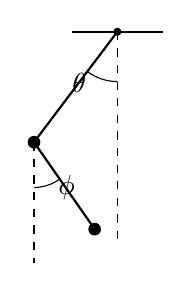
\begin{tikzpicture}[scale=1.15]
    \draw[thick] (-0.5,0) -- (0.5,0);
    \fill (0,0) circle (0.045);
    \draw[dashed] (0,0) -- (0,-2.3);
    \draw[thick] (0,0) -- (-0.92,-1.22);
    \fill (-0.92,-1.22) circle (0.07);
    \draw[dashed] (-0.92,-1.22) -- (-0.92,-2.55);
    \draw[thick] (-0.92,-1.22) -- (-0.25,-2.18);
    \fill (-0.25,-2.18) circle (0.07);
    \draw (0,-0.55) arc (-90:-127:0.55);
    \node at (-0.42,-0.56) {$\theta$};
    \draw (-0.92,-1.72) arc (-90:-55:0.48);
    \node at (-0.56,-1.72) {$\phi$};
  \end{tikzpicture}
  \caption{Generalized angular coordinates for a double pendulum.}
\end{figure}

Changing variables is similarly efficient: transform one Lagrangian and then
derive its equations, rather than transforming every force equation
separately.

\begin{classroomqa}
  \audiencequestion{Is the double pendulum essentially another three-body
  system, such as Sun, Earth, and Moon, with one body treated as an anchor?
  \lecturetimestamp{01:45:06--01:45:25}}
  \lecturerresponse{That analogy captures the hierarchy, although the rods
  impose different constraints.  In either case a very massive or fixed
  component can be treated as the reference structure in an approximation.}
\end{classroomqa}

\begin{classroomqa}
  \audiencequestion{The double pendulum uses \(T-V\), though more general
  Lagrangians were just emphasized.  When is \(T-V\) valid?
  \lecturetimestamp{01:46:08--01:46:58}}
  \lecturerresponse{For ordinary nonrelativistic particles viewed in an
  inertial frame, with no magnetic velocity coupling, the familiar form
  applies.  Rotating frames, relativistic systems, and magnetic fields require
  more general terms.}
\end{classroomqa}

\begin{classroomqa}
  \audiencequestion{Do collisions fall outside this description?
  \lecturetimestamp{01:47:00--01:48:05}}
  \lecturerresponse{Elastic collisions arise from short-range forces and
  therefore from potentials.  Inelastic collisions remain mechanical at the
  microscopic level, but energy enters internal vibrations, deformation, and
  heat.  A center-of-mass description that omits those degrees of freedom is
  incomplete.}
\end{classroomqa}

\begin{classroomqa}
  \audiencequestion{Can a baseball struck by a bat be analyzed with
  \(F=ma\)?
  \lecturetimestamp{01:48:05--01:48:33}}
  \lecturerresponse{Only at a coarse level.  A complete account must follow
  deformation, heating, possible damage to the ball, and perhaps a breaking
  bat.  Those internal degrees of freedom are why a realistic impact is much
  harder than a point-particle collision.}
\end{classroomqa}

\begin{classroomqa}
  \audiencequestion{What about an extended rigid body?
  \lecturetimestamp{01:48:34--01:49:00}}
  \lecturerresponse{Rigid bodies can be studied either with Newtonian methods
  or with a \(T-V\) Lagrangian written in translational and rotational
  coordinates.  Constructing that Lagrangian is a useful exercise.}
\end{classroomqa}

\begin{classroomqa}
  \audiencequestion{Does the quantum energy--time uncertainty relation mean
  that energy is not strictly conserved?
  \lecturetimestamp{01:49:01--01:49:29}}
  \lecturerresponse{No.  Energy can be strictly conserved.  The relation says
  that resolving energy with high accuracy requires observation over a long
  time; it does not replace the conservation law.}
\end{classroomqa}

\begin{classroomqa}
  \audiencequestion{Are Newtonian and Lagrangian mechanics logically
  equivalent?
  \lecturetimestamp{01:49:36--01:50:07}}
  \lecturerresponse{They are equivalent within the ordinary domain where both
  formulations apply.  One can nevertheless invent Lagrangians whose equations
  do not resemble the elementary form \(m\ddot x=F(x)\).}
\end{classroomqa}

\section{A Coordinate-Dependent Kinetic Term}

Consider the deliberately unfamiliar example
\begin{equation}
  L=\frac12q^2\dot q^2-\frac12q^2.
  \label{eq:l5-nonstandard-l}
\end{equation}
It is a valid Lagrangian with a coordinate-dependent kinetic coefficient.  One
could also consider velocity-linear terms such as \(q\dot q\); in this
one-dimensional example that particular term is a total derivative and would
not alter the equations of motion.

The canonical momentum is
\begin{equation}
  p=\frac{\partial L}{\partial\dot q}=q^2\dot q,
  \label{eq:l5-nonstandard-p}
\end{equation}
so
\begin{equation}
  \dot p=q^2\ddot q+2q\dot q^2,
  \qquad
  \frac{\partial L}{\partial q}=q\dot q^2-q.
  \label{eq:l5-nonstandard-derivatives}
\end{equation}
The equation of motion is therefore
\begin{equation}
  q^2\ddot q+q\dot q^2=-q.
  \label{eq:l5-nonstandard-eom}
\end{equation}

\begin{figure}[htbp]
  \centering
  
\includegraphics[width=0.80\textwidth]{lecture_05_figure_06.png}
  \caption{The differentiated momentum in the coordinate-dependent kinetic
  example.}
  \lectureframe{01:52:32}
\end{figure}

\begin{classroomqa}
  \audiencequestion{Can the equation be divided by \(q\)?
  \lecturetimestamp{01:53:22--01:53:39}}
  \lecturerresponse{Only where \(q\neq0\).  At \(q=0\) the kinetic coefficient
  and Legendre map are degenerate, so division would discard a singular point
  that needs separate treatment.}
\end{classroomqa}

The Hamiltonian is
\begin{align}
  H&=p\dot q-L
  \notag\\
   &=q^2\dot q^2-
     \left(\frac12q^2\dot q^2-\frac12q^2\right)
  \notag\\
   &=\frac12q^2\dot q^2+\frac12q^2.
  \label{eq:l5-nonstandard-h}
\end{align}

\begin{classroomqa}
  \audiencequestion{May \(q^2\dot q^2/2\) still be called the kinetic energy?
  \lecturetimestamp{01:54:41--01:55:07}}
  \lecturerresponse{Yes.  In this worked example the Hamiltonian again looks
  like a positive kinetic term plus a potential term.  The point is that the
  formal definitions worked without first assuming the elementary constant
  mass form.}
\end{classroomqa}

\section{Dissipation and the Deeper Origin of the Formalism}

\begin{classroomqa}
  \audiencequestion{How is friction included in a Lagrangian?
  \lecturetimestamp{01:55:09--01:56:17}}
  \lecturerresponse{Not as a fundamental force in the simple closed
  finite-degree-of-freedom system considered here.  Macroscopic friction is a
  statistical effect of enormous numbers of microscopic degrees of freedom.
  Those atoms still obey the underlying mechanics, but a reduced description
  that does not track them displays dissipation.}
\end{classroomqa}

\begin{classroomqa}
  \audiencequestion{How did Hamilton arrive at his formulation?
  \lecturetimestamp{01:56:22--01:56:37}}
  \lecturerresponse{No historical derivation was offered here.  The important
  task for the present course is to understand how the formulation works.}
\end{classroomqa}

\begin{classroomqa}
  \audiencequestion{Is there a more general recipe for obtaining a Lagrangian
  when it is not visibly \(T-V\)?
  \lecturetimestamp{01:56:43--01:58:54}}
  \lecturerresponse{Experiment, an informed guess, a symmetry principle, or
  reconstruction from desired equations can supply the function.  Asking the
  calculus itself where its input comes from is like asking the definition of
  a derivative where \(f(x)\) came from.  The calculus tells us what to do once
  the function is specified.  Why nature's closed systems conform to this
  abstract structure is answered at a deeper level by quantum mechanics.}
\end{classroomqa}

This point connects to the opening themes of the course.  Fundamental
Hamiltonian evolution is deterministic and reversible in the sense that
trajectories do not merge and information is not simply destroyed.  The
relation between that property and the phase-space formulation will be
developed in stages.

\begin{classroomqa}
  \audiencequestion{Did variational calculus merely work backward from the
  desired classical equations, and does quantum mechanics obtain its
  Lagrangian the same way?
  \lecturetimestamp{01:59:37--02:01:07}}
  \lecturerresponse{In the elementary classical construction, one can indeed
  choose an action whose stationary paths reproduce the known equations.  The
  logical order in quantum mechanics is different: it begins naturally with
  the Hamiltonian and can work toward a Lagrangian description.  The
  Hamiltonian is more intuitive there, even though it first appears abstract
  in classical mechanics.}
\end{classroomqa}

\begin{classroomqa}
  \audiencequestion{Can quantum mechanics describe friction?
  \lecturetimestamp{02:01:08--02:02:05}}
  \lecturerresponse{Yes, but a fundamental description must include the
  degrees of freedom of the environment.  A particle moving through a viscous
  fluid cannot be described completely without the particles of the fluid.
  Friction is the complicated collective effect that emerges when those
  degrees of freedom are not followed individually.}
\end{classroomqa}
